\section{Chemical reactions}

\subsection{Reactions and CRN}
A reaction is a set of reactants, a set of products, and a number $\kappa$ representing the speed of the reaction. Each reactant and product is some quantity of a species which can be modelled as:  
\begin{minted}{haskell}
    type Reaction = Rxn of Map<species, float> * Map<species, float> * float
\end{minted}
Where the maps map a species to its concentration, the first map is the reactants, the second map is the products and the final float is $\kappa$.

Then \texttt{CRN} can be defined as the union of all the reactions, which can be stored in a reaction list:
\begin{minted}{haskell}
    type CRN = Reaction List
\end{minted}

\subsection{Parser}

For chemical reactions we did actually implement a parser that can parse a string of chemical reactions. However we did not ever use it as the as our compiler takes an AST and compiles it directly to a list of our \texttt{F\#} type \texttt{Rxn(r,p,c)}. Therefore there is no need for a parser for the reactions. % The grammer for the parser can be seen in the appendix

\subsection{Simulation}
The system of ODE's that we want to simulate describes the rate of change of concentration for a species \( S \) within a CRN. The equation is:
\begin{equation}\label{eq:diff}
    \frac{d[S]}{dt} = \sum_{\forall \text{rxn} \in \text{CRN}} \kappa(\text{rxn}) \cdot \text{netChange}(S,\text{rxn}) \cdot \prod_{\forall R \in \text{reactants}(\text{rxn})} [R]^{m_{\text{rxn}}(R)}(t)
\end{equation}

This can be broken down into its components and translated to code. The most important part is of course that the simulation is a discretization of the continuous system. Here, $\frac{dS}{dt}$ is replaced by $\frac{\Delta S}{\Delta t}$ and $\Delta t$ is moved to the other side of the equation. The resulting equation can then be reformulated to use matrix operations, which in practice are highly optimized:

\[
\Delta \mathbf{S}(t) = \mathbf{N} \cdot \mathbf{v}(t)
\]
Where:
\begin{itemize}
    \item \( \mathbf{N} \) is the net change matrix, and each element \( \mathbf{N}_{ij} \) represents the scaled net change in species \( i \) due to reaction \( j \), including the reaction rate \( \kappa \). 
% \begin{minted}{haskell}
% let genNetChangeMatrix (crn : CRN) (sl : species List) = 
%     Matrix.ofJaggedList (List.foldBack (fun s st -> 
%         genNetChangeList crn s :: st) sl [])
% \end{minted}
%Where \texttt{genNetChangeList} multiplies the reaction speed $c$ with the \texttt{netChange}:
% \begin{minted}{haskell}
%     let genNetChangeList (crn : CRN) (s : species) = 
%         (List.foldBack (fun (Rxn(r,p,c)) st -> 
%             c * (calcNetChange (Rxn(r,p,c)) s) :: st) crn [])
% \end{minted}
%and the \texttt{netChange} is calculated by:
% \begin{minted}{haskell}
%     let calcNetChange (Rxn(r, p, c)) (s: species) = 
%         (getValue p s) - (getValue r s) 

% \end{minted}

    \item \( \mathbf{v}(t) \) is a vector where each component corresponds to the product of the concentrations of reactants raised to their stoichiometric coefficients for each reaction at time \( t \). This vector depends on $S(t)$ and is therefore calculated at each time step. It plays the same role as the product in equation \ref{eq:diff}. 
    %This vector is computed by:
% \begin{minted}{haskell}
% let calcReactionProducts (state : State) (crn : CRN) = 
%     vector (
%         List.map (fun (Rxn(r, _, _)) ->
%             Map.fold (fun s coeff prod -> 
%                 prod * (state |> Map.find s) ** coeff) 1.0 r
%         ) crn
%     )
% \end{minted}
    \item $\Delta \mathbf{S}$ is a vector containing the change for each species at some time. This vector is added to the current State which yields the simulated state at time $t+\Delta t$. 
    %This is calculated in the following way
    %     \begin{minted}{haskell}
    %     let calcDerivatives netChangeMatrix reactionProduct timestep =
    %         timestep * (netChangeMatrix * reactionProduct) 
    % \end{minted}
\end{itemize}

We wanted to further optimize the calculation of \(\mathbf{v}(t)\), by using the logarithm to transform it into a dot-product, however this led to problems since it is possible for concentrations to be zero. In summary, the updated state can be calculated by transforming the current state to the $\mathbf{v}$ vector and performing a dot product with a constant matrix defined in preprocessing. Lastly, the infinite sequence of states can then be calculated using a \texttt{Seq.unfold} similar to the code for the interpreter, using the function for updating a state to the next. See the code for more details. 

\subsection{Visualization}
Since this simulation results in a sequence of states, just like the interpreter from the prior section, we can use the visualization code from the interpreter to visualize the simulation. The plots for this section can be seen in appendix \ref{sec:compiler_plots}.

\subsection{Testing}
As with the interpreter, all the modules from Table 1 in the paper were tested individually for the simulator. All of them passed all tests, except the \texttt{cmp} and \texttt{sub} modules. For \texttt{cmp} we encountered for some values that the binary flags \texttt{Xegty} among the other, have problems reaching 0 and 1. For \texttt{sub} we encountered some of the problems also described in the article. The \texttt{sub} module is by far the module with highest error and when \texttt{X} is very close to or equal to \texttt{Y} in \texttt{X-Y} the error becomes very high. This however is expected so there is really no reason to try and fix this. More on this in the assessment.

\subsection{Assessment}
As a whole, we are pleased with the outcome of this section. The optimization of the simulation using matrix operations was especially rewarding. The tests also proved helpful, both for finding and fixing bugs, but also for figuring out that the simulation of the \texttt{cmp} module does not behave as expected. When simulating \texttt{cmp}, for example \texttt{cmp[a,b]}, the error becomes larger as the fraction $\frac{a}{b}$ goes to 1. Even if we make the requirements easier, \texttt{cmp} will still fail given two large enough neighbouring numbers. This is illustrated in the following figure:
\begin{figure}[H]
    \centering
    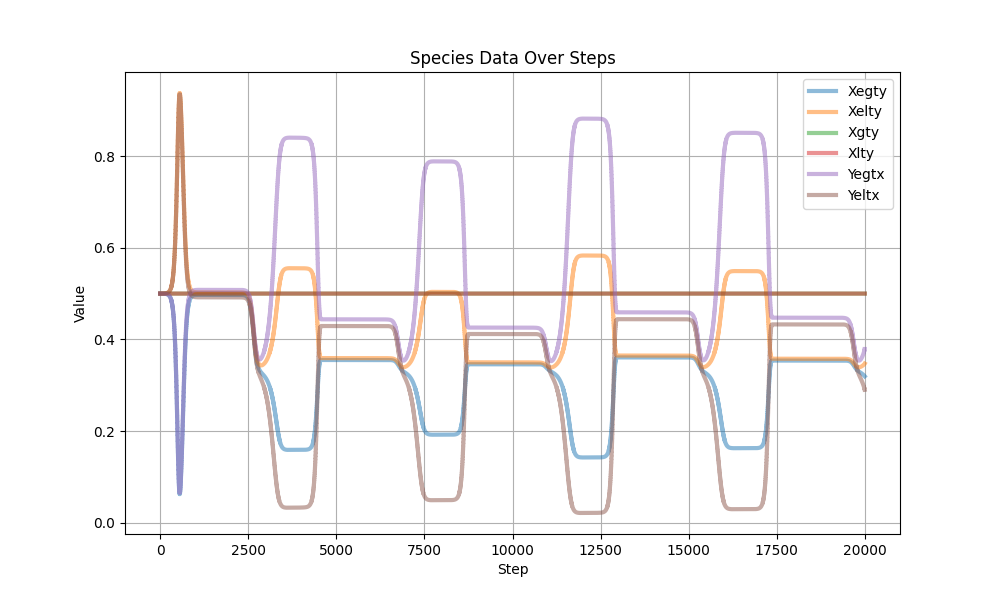
\includegraphics[scale=0.22]{report/figures/cmpbad.png}
    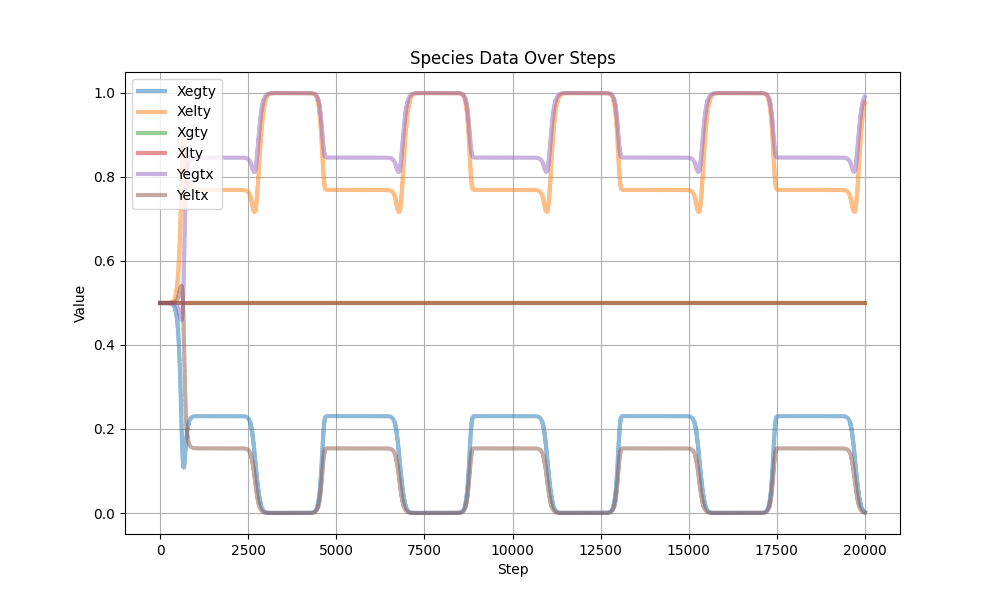
\includegraphics[scale=0.22]{report/figures/cmpgood.png}
    \caption{Plot of compare, where the right one does well on the numbers 1 and 5, while the left one does a bit poorer on 45 and 46.}
\end{figure}

The only negative part was that we never had a reason to use the parser for chemical reactions (point 9), which led to it feeling less rewarding and more like only an obligation.
